%%%%%%%%%%%%%%%%%%%%%%%%%%%%% Define Article %%%%%%%%%%%%%%%%%%%%%%%%%%%%%%%%%%
\documentclass{article}
%%%%%%%%%%%%%%%%%%%%%%%%%%%%%%%%%%%%%%%%%%%%%%%%%%%%%%%%%%%%%%%%%%%%%%%%%%%%%%%

%%%%%%%%%%%%%%%%%%%%%%%%%%%%% Using Packages %%%%%%%%%%%%%%%%%%%%%%%%%%%%%%%%%%
\usepackage{geometry}
\usepackage{graphicx}
\usepackage{amssymb}
\usepackage{amsmath}
\usepackage{amsthm}
\usepackage{empheq}
\usepackage{mdframed}
\usepackage{booktabs}
\usepackage{lipsum}
\usepackage{graphicx}
\usepackage{color}
\usepackage{psfrag}
\usepackage{pgfplots}
\usepackage{bm}

\usepackage{pdfpages}
%%%%%%%%%%%%%%%%%%%%%%%%%%%%%%%%%%%%%%%%%%%%%%%%%%%%%%%%%%%%%%%%%%%%%%%%%%%%%%%

% Other Settings

%%%%%%%%%%%%%%%%%%%%%%%%%% Page Setting %%%%%%%%%%%%%%%%%%%%%%%%%%%%%%%%%%%%%%%
\geometry{a4paper}

%%%%%%%%%%%%%%%%%%%%%%%%%% Define some useful colors %%%%%%%%%%%%%%%%%%%%%%%%%%
\definecolor{ocre}{RGB}{243,102,25}
\definecolor{mygray}{RGB}{243,243,244}
\definecolor{deepGreen}{RGB}{26,111,0}
\definecolor{shallowGreen}{RGB}{235,255,255}
\definecolor{deepBlue}{RGB}{61,124,222}
\definecolor{shallowBlue}{RGB}{235,249,255}
%%%%%%%%%%%%%%%%%%%%%%%%%%%%%%%%%%%%%%%%%%%%%%%%%%%%%%%%%%%%%%%%%%%%%%%%%%%%%%%

%%%%%%%%%%%%%%%%%%%%%%%%%% Define an orangebox command %%%%%%%%%%%%%%%%%%%%%%%%
\newcommand\orangebox[1]{\fcolorbox{ocre}{mygray}{\hspace{1em}#1\hspace{1em}}}
%%%%%%%%%%%%%%%%%%%%%%%%%%%%%%%%%%%%%%%%%%%%%%%%%%%%%%%%%%%%%%%%%%%%%%%%%%%%%%%

%%%%%%%%%%%%%%%%%%%%%%%%%%%% English Environments %%%%%%%%%%%%%%%%%%%%%%%%%%%%%
\newtheoremstyle{mytheoremstyle}{3pt}{3pt}{\normalfont}{0cm}{\rmfamily\bfseries}{}{1em}{{\color{black}\thmname{#1}~\thmnumber{#2}}\thmnote{\,--\,#3}}
\newtheoremstyle{myproblemstyle}{3pt}{3pt}{\normalfont}{0cm}{\rmfamily\bfseries}{}{1em}{{\color{black}\thmname{#1}~\thmnumber{#2}}\thmnote{\,--\,#3}}
\theoremstyle{mytheoremstyle}
\newmdtheoremenv[linewidth=1pt,backgroundcolor=shallowGreen,linecolor=deepGreen,leftmargin=0pt,innerleftmargin=20pt,innerrightmargin=20pt,]{theorem}{Theorem}[section]
\theoremstyle{mytheoremstyle}
\newmdtheoremenv[linewidth=1pt,backgroundcolor=shallowBlue,linecolor=deepBlue,leftmargin=0pt,innerleftmargin=20pt,innerrightmargin=20pt,]{definition}{Definition}[section]
\theoremstyle{myproblemstyle}
\newmdtheoremenv[linecolor=black,leftmargin=0pt,innerleftmargin=10pt,innerrightmargin=10pt,]{problem}{Problem}[section]
%%%%%%%%%%%%%%%%%%%%%%%%%%%%%%%%%%%%%%%%%%%%%%%%%%%%%%%%%%%%%%%%%%%%%%%%%%%%%%%

%%%%%%%%%%%%%%%%%%%%%%%%%%%%%%% Plotting Settings %%%%%%%%%%%%%%%%%%%%%%%%%%%%%
\usepgfplotslibrary{colorbrewer}
\pgfplotsset{width=8cm,compat=1.9}
%%%%%%%%%%%%%%%%%%%%%%%%%%%%%%%%%%%%%%%%%%%%%%%%%%%%%%%%%%%%%%%%%%%%%%%%%%%%%%%

%%%%%%%%%%%%%%%%%%%%%%%%%%%%%%% Title & Author %%%%%%%%%%%%%%%%%%%%%%%%%%%%%%%%
\title{Chapter 4.1 Integration}
\author{Aarav Yadav}
%%%%%%%%%%%%%%%%%%%%%%%%%%%%%%%%%%%%%%%%%%%%%%%%%%%%%%%%%%%%%%%%%%%%%%%%%%%%%%%

\begin{document}
    \maketitle

    \setcounter{section}{4}


    \begin{definition}[Definition of Antiderivatice]
        A function F is an antiderivative of f on an interval I when F'(x) = f(x) for all x in I
    \end{definition}

    \begin{theorem}[Representation of Antiderivatives]
        If F is an antiderivatice of f on an interval I, then G is an antiderivative of f on the
        interval I if an only if G is of the form $ G(x) = F(x) + C $ for all x in I where C is constant.
    \end{theorem}
    
    \begin{problem}[Solving a Differential Equation]
        Find the general solution of the differential equation $ y' = 2 $
    \end{problem}
    
    \begin{problem}[Describing Antiderivatives]
        Solve. $ \int_{}^{} 3x dx $ 
    \end{problem}

    \begin{problem}[Rewriting Before Integration]
        Rewrite, Integrate, Simplify
        \begin{itemize}
            \item $ \int_{}^{} 1/x^{3} dx $
            \item $ \int_{}^{} \sqrt[]{x} dx $
        \end{itemize} 
    \end{problem}
    
    \begin{problem}[Integrating Polynomial Functions]
        Solve.

        \begin{itemize}
            \item $ \int_{}^{} dx $
            \item $ \int_{}^{} (x+2) dx $
            \item $ \int_{}^{} (3x^4 - 5x^2 + x) dx $ 
        \end{itemize}
    \end{problem}

    \begin{problem}[Rewriting Before Integrating]
        Solve. $ \int_{}^{} \frac{(x+1)}{(\sqrt[]{x})}  dx$
    \end{problem}

    \begin{problem}[Rewriting Before Integrating]
        $ \int_{}^{} \frac{sin(x)}{cos^2(x)} dx$
    \end{problem}

    \begin{problem}[Rewriting Before Integrating]
        Rewrite, Integrate, Simplify.
        \begin{itemize}
            \item $ \int_{}^{} \frac{2}{\sqrt[]{x}} dx$
            \item $ \int_{}^{} (t^2 + 1)^2 dt$
            \item $ \int_{}^{} \frac{x^3+3}{x^2} dx$
            \item $ \int_{}^{} \sqrt[3]{x} (x - 4) dx$
        \end{itemize}
    \end{problem}

    \begin{definition}[Particular Solution]
        In many applications of integration, you are given enough information to determine a particular solution.
        To do this, you need only know the value of y = F(x) for one value of x. This information is 
        called an \textbf{initial condition}.
    \end{definition}

    \begin{definition}[Initial Condition]
        The value of y = F(x) for one value of x.
    \end{definition}

    \begin{problem}[Finding a Particular Solution]
        Find the \textbf{general solution}: $ F'(x) = e^x $
        
        and find the particular solution that satisfies the \textbf{initial condition}: $ F(0) = 3 $
    \end{problem}

    NOTE: So far in this section, you have been using x as the variable of integration.
    In applications, it is often convenient to use a different variable. For instance, in the next
    example, involving \textit{time}, the \textbf{variable of integration} is t.

    \begin{problem}[Solving a Vertical Motion Problem]
        A ball is thrown upward with an initial velocity of 64 feet per second from an initial
        height of 80 feet. (a) Find the \textbf{position function giving the height s as a function of the time t}.
        (b) \textbf{When} does the ball hit \textbf{the ground}?
    \end{problem}

    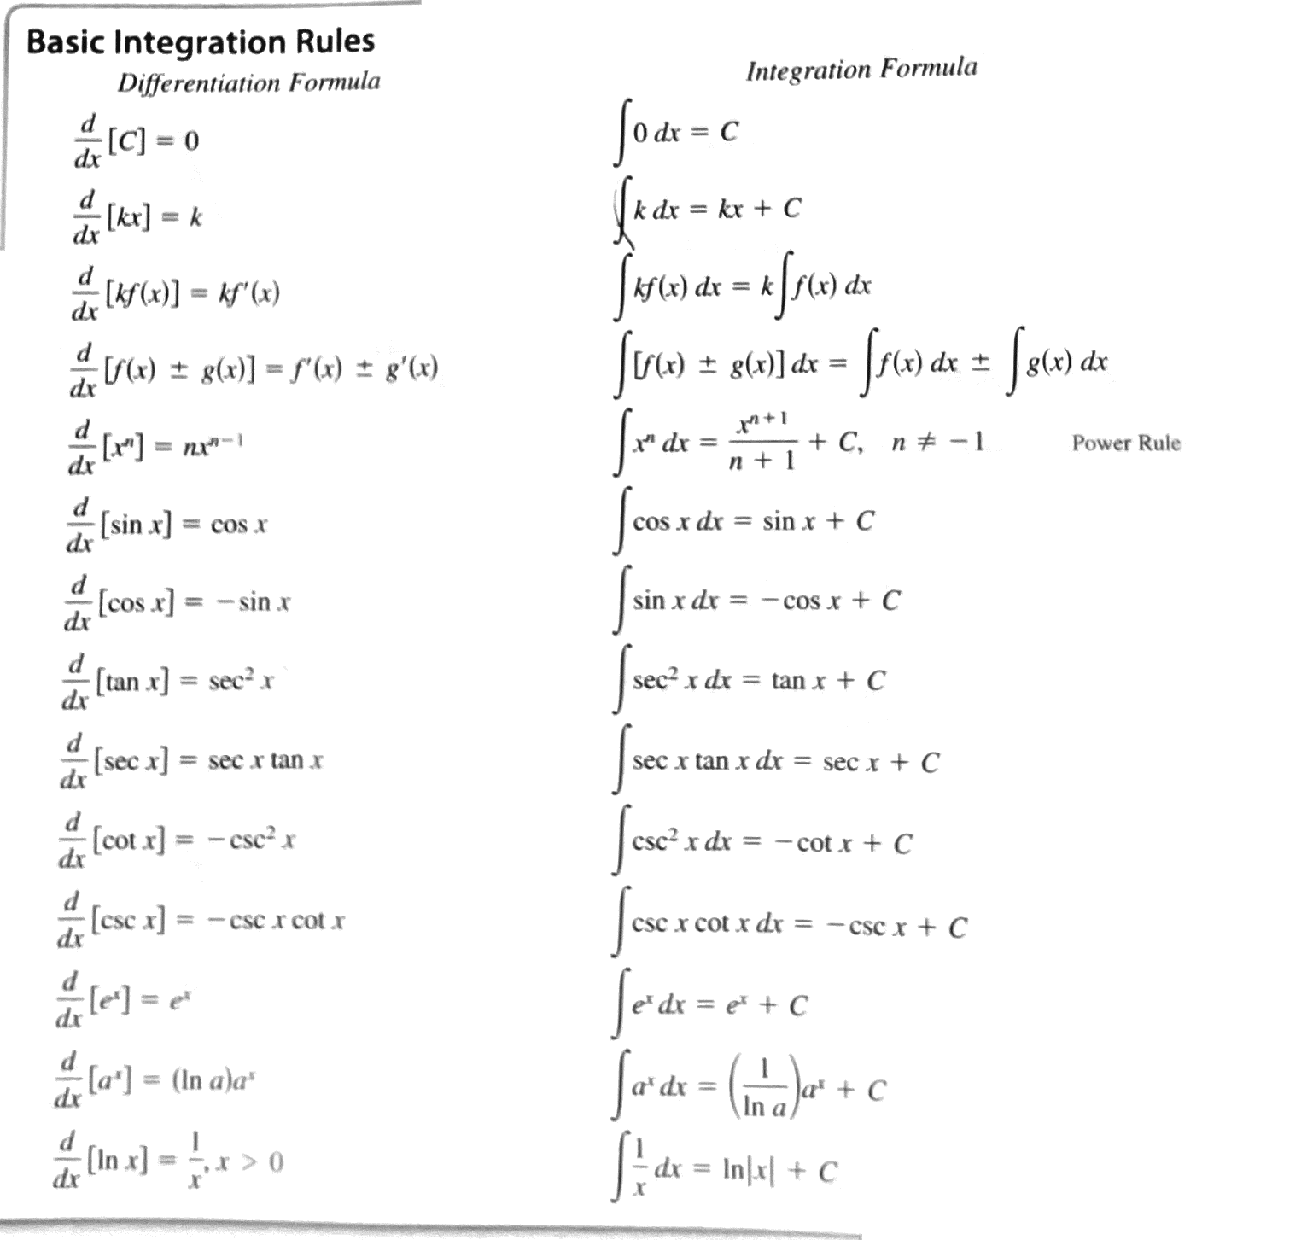
\includepdf[pages=-]{Basic Integration Rules.pdf}

\end{document}